% Template adapted from https://github.com/jgm/pandoc-templates/blob/master/default.latex
% To be used with XeLaTex in memoiR
%%%%%%%%%%%%%%%%%%%%%%%%%%%%%%%%%%%%%%%%%%%%%%%%%%%%%%%%%%%%%%%%%%%%%%%%%%%%%%%%%%%%%%%%%

% Options for packages loaded elsewhere
\PassOptionsToPackage{unicode=true}{hyperref}
\PassOptionsToPackage{hyphens}{url}
\PassOptionsToPackage{dvipsnames,svgnames*,x11names*}{xcolor}
% Right to left support


\documentclass[
  11pt,
  italian,
  a4paper,
  extrafontsizes,onecolumn,openright
  ]{memoir}

% Double (or whatever) spacing

% Math
\usepackage{amssymb, amsmath}
% mathspec: arbitrary math fonts
\usepackage{unicode-math}
\defaultfontfeatures{Scale=MatchLowercase}
\defaultfontfeatures[\rmfamily]{Ligatures=TeX,Scale=1}

% Fonts
\usepackage{lmodern}
\usepackage{fontspec}

% Main font
% Specific sanserif font
% Specific monotype font
\setmonofont[Scale=0.85]{Inconsolata}
% Specific math font
% Chinese, Japanese, Corean fonts

% Use upquote for straight quotes in verbatim environments
\usepackage{upquote}
% Use microtype
\usepackage[]{microtype}
\UseMicrotypeSet[protrusion]{basicmath} % disable protrusion for tt fonts

% Verbatim in note

% Color links
\usepackage{xcolor}

% Strikeout

% Necessary for code chunks
\usepackage{color}
\usepackage{fancyvrb}
\newcommand{\VerbBar}{|}
\newcommand{\VERB}{\Verb[commandchars=\\\{\}]}
\DefineVerbatimEnvironment{Highlighting}{Verbatim}{commandchars=\\\{\}}
% Add ',fontsize=\small' for more characters per line
\usepackage{framed}
\definecolor{shadecolor}{RGB}{248,248,248}
\newenvironment{Shaded}{\begin{snugshade}}{\end{snugshade}}
\newcommand{\AlertTok}[1]{\textcolor[rgb]{0.94,0.16,0.16}{#1}}
\newcommand{\AnnotationTok}[1]{\textcolor[rgb]{0.56,0.35,0.01}{\textbf{\textit{#1}}}}
\newcommand{\AttributeTok}[1]{\textcolor[rgb]{0.77,0.63,0.00}{#1}}
\newcommand{\BaseNTok}[1]{\textcolor[rgb]{0.00,0.00,0.81}{#1}}
\newcommand{\BuiltInTok}[1]{#1}
\newcommand{\CharTok}[1]{\textcolor[rgb]{0.31,0.60,0.02}{#1}}
\newcommand{\CommentTok}[1]{\textcolor[rgb]{0.56,0.35,0.01}{\textit{#1}}}
\newcommand{\CommentVarTok}[1]{\textcolor[rgb]{0.56,0.35,0.01}{\textbf{\textit{#1}}}}
\newcommand{\ConstantTok}[1]{\textcolor[rgb]{0.00,0.00,0.00}{#1}}
\newcommand{\ControlFlowTok}[1]{\textcolor[rgb]{0.13,0.29,0.53}{\textbf{#1}}}
\newcommand{\DataTypeTok}[1]{\textcolor[rgb]{0.13,0.29,0.53}{#1}}
\newcommand{\DecValTok}[1]{\textcolor[rgb]{0.00,0.00,0.81}{#1}}
\newcommand{\DocumentationTok}[1]{\textcolor[rgb]{0.56,0.35,0.01}{\textbf{\textit{#1}}}}
\newcommand{\ErrorTok}[1]{\textcolor[rgb]{0.64,0.00,0.00}{\textbf{#1}}}
\newcommand{\ExtensionTok}[1]{#1}
\newcommand{\FloatTok}[1]{\textcolor[rgb]{0.00,0.00,0.81}{#1}}
\newcommand{\FunctionTok}[1]{\textcolor[rgb]{0.00,0.00,0.00}{#1}}
\newcommand{\ImportTok}[1]{#1}
\newcommand{\InformationTok}[1]{\textcolor[rgb]{0.56,0.35,0.01}{\textbf{\textit{#1}}}}
\newcommand{\KeywordTok}[1]{\textcolor[rgb]{0.13,0.29,0.53}{\textbf{#1}}}
\newcommand{\NormalTok}[1]{#1}
\newcommand{\OperatorTok}[1]{\textcolor[rgb]{0.81,0.36,0.00}{\textbf{#1}}}
\newcommand{\OtherTok}[1]{\textcolor[rgb]{0.56,0.35,0.01}{#1}}
\newcommand{\PreprocessorTok}[1]{\textcolor[rgb]{0.56,0.35,0.01}{\textit{#1}}}
\newcommand{\RegionMarkerTok}[1]{#1}
\newcommand{\SpecialCharTok}[1]{\textcolor[rgb]{0.00,0.00,0.00}{#1}}
\newcommand{\SpecialStringTok}[1]{\textcolor[rgb]{0.31,0.60,0.02}{#1}}
\newcommand{\StringTok}[1]{\textcolor[rgb]{0.31,0.60,0.02}{#1}}
\newcommand{\VariableTok}[1]{\textcolor[rgb]{0.00,0.00,0.00}{#1}}
\newcommand{\VerbatimStringTok}[1]{\textcolor[rgb]{0.31,0.60,0.02}{#1}}
\newcommand{\WarningTok}[1]{\textcolor[rgb]{0.56,0.35,0.01}{\textbf{\textit{#1}}}}

% Listings package

% Tables
\usepackage{longtable,booktabs,tabu}
% Fix footnotes in tables (requires footnote package)
\IfFileExists{footnote.sty}{\usepackage{footnote}\makesavenoteenv{longtable}}{}

% Graphics
\usepackage{graphicx,grffile}
\graphicspath{{images/}}
\makeatletter
\def\maxwidth{\ifdim\Gin@nat@width>\linewidth\linewidth\else\Gin@nat@width\fi}
\def\maxheight{\ifdim\Gin@nat@height>\textheight\textheight\else\Gin@nat@height\fi}
\makeatother
% Scale images if necessary, so that they will not overflow the page
% margins by default, and it is still possible to overwrite the defaults
% using explicit options in \includegraphics[width, height, ...]{}
\setkeys{Gin}{width=\maxwidth,height=\maxheight,keepaspectratio}

% Prevent overfull lines
\setlength{\emergencystretch}{3em}  
\providecommand{\tightlist}{%
  \setlength{\itemsep}{0pt}\setlength{\parskip}{0pt}}

% Number sections for memoir (secnumdepth counter is ignored)
\setsecnumdepth{section}

% Set default figure placement to htbp
\makeatletter
\def\fps@figure{htbp}
\makeatother

% Spacing in lists
\usepackage{enumitem}

% Polyglossia
\usepackage{polyglossia}
\setmainlanguage{it}
\setotherlanguage{en-US}

% BibLaTeX
\usepackage[backend=biber,style=authoryear-ibid,isbn=false,backref=true,giveninits=true,uniquename=init,maxcitenames=2,maxbibnames=150,sorting=nyt,sortcites=false,style=apa]{biblatex}
\addbibresource{refs.bib}

% cslreferences environment required by pandoc > 2.7



%%%%%%%%%%%%%%%%%%%%%%%%%%%%%%%%%%%%%%%%%%%%%%%%%%%%%%%%%%
% memoiR format

% Chapter Summary environment 
\usepackage[tikz]{bclogo}
\newenvironment{Summary}
  {\begin{bclogo}[logo=\bctrombone, noborder=true, couleur=lightgray!50]{In breve}\parindent0pt}
  {\end{bclogo}}
% Syntax:
%
%```{block, type='Summary'}
% Deliver message here.
% ```

% scriptsize code 
\let\oldverbatim\verbatim
\def\verbatim{\oldverbatim\scriptsize}
% Applies to code blocks and R code results
% code chunk options size='scriptsize' applies only to R code and results
% if the code chunk sets a different size, \def\verbatim{...} is prioritary for code results 


% Layout
%%%%%%%%%%%%%%%%%%%%%%%%%%%%%%%%%%%%%%%%%%%%%%%%%%%%%%%%%%

% Based on memoir, style companion
\newcommand{\MemoirChapStyle}{daleif1}
\newcommand{\MemoirPageStyle}{Ruled}

% Space between paragraphs
\usepackage{parskip}
  \abnormalparskip{3pt}

% Adjust margin paragraphs vertical position
\usepackage{marginfix}


% Margins
%%%%%%%%%%%%%%%%%%%%%%%%%%%%%%%%%%%%%%%

% allow use of '-',+','/' ans '*' to make simple length computation
\usepackage{calc}

% Full-width figures utilities
\newlength\widthw % full width
\newlength{\rf}
\newcommand*{\definesHSpace}{
  \strictpagecheck % slower but efficient detection of odd/even pages
  \checkoddpage
  \ifoddpage
  \setlength{\rf}{0mm}
  \else
  \setlength{\rf}{\marginparsep+\marginparwidth}
  \fi
}

\makeatletter
% 1" margins for the front matter.
\newcommand*{\SmallMargins}{
  \setlrmarginsandblock{1.5in}{1.5in}{*}
  \setmarginnotes{0.1in}{0.1in}{0.1in}
 \setulmarginsandblock{1.5in}{1in}{*}
  \checkandfixthelayout
  \ch@ngetext
  \clearpage
  \setlength{\widthw}{\textwidth+\marginparsep+\marginparwidth}
  \footnotesatfoot
  \chapterstyle{\MemoirChapStyle}  % Chapter and page styles must be recalled
  \pagestyle{\MemoirPageStyle}
}

% 3" outer margin for the main matter
\newcommand{\LargeMargins}{\SmallMargins}
\makeatother

% Figure captions and footnotes in outer margins


% Main title page with filigrane
%%%%%%%%%%%%%%%%%%%%%%%%%%%%%%%%%%%%%%%%%%%%%%%%%%%%%%%%%%

% Text blocks
\usepackage[absolute,overlay]{textpos}
  \setlength{\TPHorizModule}{1mm}
  \setlength{\TPVertModule}{1mm}

\newcommand{\MainTitlePage}[2]{
  \SmallMargins % Margins
  \pagestyle{empty} % No header/footer
  \textblockorigin{\stockwidth-\paperwidth-\trimedge}{\trimtop} % recto
  \begin{textblock*}{2mm}(\spinemargin/2,\uppermargin/2)
    \rule{1pt}{\paperheight-\uppermargin}
  \end{textblock*}
  \begin{textblock*}{\paperwidth*2/3}(\paperwidth/5, \paperheight/5)
    \flushright
    \begin{Spacing}{3}
      {\fontfamily{qtm}\selectfont\fontsize{45}{45}\selectfont\textsc{\thetitle}}
    \end{Spacing}
  \end{textblock*}
    \begin{textblock*}{\paperwidth*2/3}(\paperwidth/5, \paperheight/2)
    \flushright
    {\fontfamily{qtm}\huge\theauthor}
  \end{textblock*}
    \begin{textblock*}{\paperwidth*2/3}[0, 1](\spinemargin, \uppermargin+\textheight)
    \normalfont\thedate
  \end{textblock*}
  ~\\ % Print a character or the page will not exist
  \newpage
  \textblockorigin{\trimedge}{\trimtop} % verso
  \begin{textblock*}{\textwidth}(\paperwidth-\spinemargin-\textwidth, \uppermargin)
    #1
  \end{textblock*}
  \begin{textblock*}{\textwidth}[0,1](\paperwidth-\spinemargin-\textwidth, \uppermargin+\textheight+\footskip)
    \centering
    
\includegraphics[width=\paperwidth/4]{logo}\\ \bigskip
    #2
  \end{textblock*}
  ~\\ % Print a character or the page will not exist
  \newpage
}

% Clear page and open an even one (\clearpage opens an odd one)
\newcommand{\evenpage}{
  \clearpage
  \strictpagecheck % slower but efficient detection of odd/even pages
  \checkoddpage
  \ifoddpage
    \thispagestyle{empty}
    ~\\ % Print a character or the page will not exist
    \newpage
  \else
    % do nothing
  \fi
}


%% PDF title page to insert
%%%%%%%%%%%%%%%%%%%%%%%%%%%%%%%%%%%%%%%%%%%%%%%%%%%%%%%%%%



%% Bibliography
%%%%%%%%%%%%%%%%%%%%%%%%%%%%%%%%%%%%%%%%%%%%%%%%%%%%%%%%%%

\usepackage[strict,autostyle]{csquotes}
% Repeated citation as author-year-title instead of author-title (modification of footcite:note in verbose-inote.cbx)

%% Table of Contents
%%%%%%%%%%%%%%%%%%%%%%%%%%%%%%%%%%%%%%%%%%%%%%%%%%%%%%%%%%

% fix the typesetting of the part number
\renewcommand\partnumberlinebox[2]{#2\ ---\ }


% Fonts
%%%%%%%%%%%%%%%%%%%%%%%%%%%%%%%%%%%%%%%%%%%%%%%%%%%%%%%%%%


% Hyperref comes last
%%%%%%%%%%%%%%%%%%%%%%%%%%%%%%%%%%%%%%%%%%%%%%%%%%%%%%%%%%

\usepackage{hyperref}
\hypersetup{
  pdftitle={Psicometria},
  pdfauthor={Corrado Caudek},
  colorlinks=true,
  linkcolor=Maroon,
  citecolor=Blue,
  urlcolor=Blue,
  breaklinks=true}

% Don't use monospace font for urls
\urlstyle{same}


% Title, author, date from YAML to LaTeX
%%%%%%%%%%%%%%%%%%%%%%%%%%%%%%%%%%%%%%%%%%%%%%%%%%%%%%%%%%

\title{Psicometria}

\author{Corrado Caudek}

\date{2021-10-16}


% Include headers (preamble.tex) here
%%%%%%%%%%%%%%%%%%%%%%%%%%%%%%%%%%%%%%%%%%%%%%%%%%%%%%%%%%
% Add LaTeX code into the preamble of the document here
\hyphenation{bio-di-ver-si-ty sap-lings}


%%%%%%%%%%%%%%%%%%%%%%%%%%%%%%%%%%%%%%%%%%%%%%%%%%%%%%%%%%%%%%%%%%%%%%%%%
% memoiR dalef3 chapter style 
% https://ctan.crest.fr/tex-archive/info/latex-samples/MemoirChapStyles/MemoirChapStyles.pdf
\usepackage{soul}
\definecolor{nicered}{rgb}{.647,.129,.149}
\makeatletter
\newlength\dlf@normtxtw
\setlength\dlf@normtxtw{\textwidth}
\def\myhelvetfont{\def\sfdefault{mdput}}
\newsavebox{\feline@chapter}
\newcommand\feline@chapter@marker[1][4cm]{%
  \sbox\feline@chapter{%
    \resizebox{!}{#1}{\fboxsep=1pt%
	  \colorbox{nicered}{\color{white}\bfseries\sffamily\thechapter}%
	}}%
  \rotatebox{90}{%
    \resizebox{%
	  \heightof{\usebox{\feline@chapter}}+\depthof{\usebox{\feline@chapter}}}%
	{!}{\scshape\so\@chapapp}}\quad%
  \raisebox{\depthof{\usebox{\feline@chapter}}}{\usebox{\feline@chapter}}%
 }
\newcommand\feline@chm[1][4cm]{%
  \sbox\feline@chapter{\feline@chapter@marker[#1]}%
  \makebox[0pt][l]{% aka \rlap
    \makebox[1cm][r]{\usebox\feline@chapter}%
  }}
\makechapterstyle{daleif1}{
  \renewcommand\chapnamefont{\normalfont\Large\scshape\raggedleft\so}
  \renewcommand\chaptitlefont{\normalfont\huge\bfseries\scshape\color{nicered}}
  \renewcommand\chapternamenum{}
  \renewcommand\printchaptername{}
  \renewcommand\printchapternum{\null\hfill\feline@chm[2.5cm]\par}
  \renewcommand\afterchapternum{\par\vskip\midchapskip}
  \renewcommand\printchaptertitle[1]{\chaptitlefont\raggedleft ##1\par}
}
\makeatother

\DeclareMathOperator{\Var}{Var} % Define variance operator
\DeclareMathOperator{\SD}{SD} % Define sd operator
\DeclareMathOperator{\Cov}{Cov} % Define covariance operator
\DeclareMathOperator{\Corr}{Corr} % Define correlation operator
\DeclareMathOperator{\Me}{Me} % Define mediane operator
\DeclareMathOperator{\Mo}{Mo} % Define mode operator
\DeclareMathOperator{\Bin}{Bin} % Define binomial operator
\DeclareMathOperator{\Bernoulli}{Bernoulli} % Define Bernoulli operator
\DeclareMathOperator{\Poi}{Poi} % Define Poisson operator
\DeclareMathOperator{\Uniform}{Uniform} % Define Uniform operator
\DeclareMathOperator{\Cauchy}{Cauchy} % Define Cauchy operator
\DeclareMathOperator{\elpd}{elpd} % Define elpd operator
\DeclareMathOperator{\lppd}{lppd} % Define lppd operator
\DeclareMathOperator{\LOO}{LOO} % Define LOO operator
\DeclareMathOperator{\B}{\mathscr{B}} % Define Bernoulli operator
\newcommand{\R}{\textsf{R}} % Define R programming language symbol
\newcommand{\E}{\mathbb{E}} % Define expected value operator
\newcommand{\Real}{\mathbb{R}} % Define real number operator
\newcommand{\Prob}{\mathscr{P}}
\DeclareMathOperator*{\argmin}{arg\,min} % thin space, limits on side in displays
\DeclareMathOperator*{\argmax}{arg\,max} % thin space, limits on side in displays

\raggedbottom % allow variable (ragged) site heights
\frenchspacing

\usepackage[
  labelfont=bf, 
  font={small, it} 
]{caption} 
\usepackage{upquote} % print correct quotes in verbatim-environments
\usepackage{empheq} 
\usepackage{xfrac}





\usepackage{booktabs}
\usepackage{longtable}
\usepackage{array}
\usepackage{multirow}
\usepackage{wrapfig}
\usepackage{float}
\usepackage{colortbl}
\usepackage{pdflscape}
\usepackage{tabu}
\usepackage{threeparttable}
\usepackage{threeparttablex}
\usepackage[normalem]{ulem}
\usepackage{makecell}
\usepackage{xcolor}


% End of preamble
%%%%%%%%%%%%%%%%%%%%%%%%%%%%%%%%%%%%%%%%%%%%%%%%%%%%%%%%%%


\begin{document}
\frontmatter

% Title page
%%%%%%%%%%%%%%%%%%%%%%%%%%%%%%%%%%%%%%%%%%%%%%%%%%%%%%%%%%


\MainTitlePage{Questo documento è stato realizzato con:

\begin{itemize}
  \item \LaTeX\; e la classe memoir (\url{http://www.ctan.org/pkg/memoir});
  \item $\R$ (\url{http://www.r-project.org/}) e RStudio (\url{http://www.rstudio.com/});
  \item bookdown (\url{http://bookdown.org/}) e memoiR (\url{https://ericmarcon.github.io/memoiR/}).
\end{itemize}}{Nel blog della mia pagina personale sono forniti alcuni approfondimenti degli argomenti qui trattati.

\url{https://ccaudek.github.io/caudeklab/}}


% Before Body
%%%%%%%%%%%%%%%%%%%%%%%%%%%%%%%%%%%%%%%%%%%%%%%%%%%%%%%%%%





% Contents
%%%%%%%%%%%%%%%%%%%%%%%%%%%%%%%%%%%%%%%%%%%%%%%%%%%%%%%%%%

\LargeMargins
{
\hypersetup{linkcolor=}
\setcounter{tocdepth}{2}
\tableofcontents
}


% Body
%%%%%%%%%%%%%%%%%%%%%%%%%%%%%%%%%%%%%%%%%%%%%%%%%%%%%%%%%%

\LargeMargins
\hypertarget{prefazione}{%
\chapter{Prefazione}\label{prefazione}}

\textbf{Data Science per psicologi} contiene il materiale delle lezioni dell'insegnamento di \emph{Psicometria B000286} (A.A. 2021/2022) rivolto agli studenti del primo anno del Corso di Laurea in Scienze e Tecniche Psicologiche dell'Università degli Studi di Firenze.

L'insegnamento di Psicometria si propone di fornire agli studenti un'introduzione all'analisi dei dati in psicologia.
Le conoscenze/competenze che verranno sviluppate in questo insegnamento sono quelle della \emph{Data science}, ovvero le conoscenze/competenze che si pongono all'intersezione tra statistica (ovvero, richiedono la capacità di comprendere teoremi statistici) e informatica (ovvero, richiedono la capacità di sapere utilizzare un software).

\hypertarget{la-psicologia-e-la-data-science}{%
\section*{La psicologia e la Data Science}\label{la-psicologia-e-la-data-science}}
\addcontentsline{toc}{section}{La psicologia e la Data Science}

\begin{quote}
It's worth noting, before getting started, that this material is hard. If you find yourself confused at any point, you are normal. Any sense of confusion you feel is just your brain correctly calibrating to the subject matter. Over time, confusion is replaced by comprehension {[}\ldots{]} --- Richard McElreath
\end{quote}

Sembra sensato spendere due parole su un tema che è importante per gli studenti: quello indicato dal titolo di questo Capitolo. È ovvio che agli studenti di psicologia la statistica non piace. Se piacesse, forse studierebbero Data Science e non psicologia; ma non lo fanno. Di conseguenza, gli studenti di psicologia si chiedono: ``perché dobbiamo perdere tanto tempo a studiare queste cose quando in realtà quello che ci interessa è tutt'altro?'\,' Questa è una bella domanda.

C'è una ragione molto semplice che dovrebbe farci capire perché la Data Science è così importante per la psicologia. Infatti, a ben pensarci, la psicologia è una disciplina intrinsecamente statistica, se per statistica intendiamo quella disciplina che studia la variazione delle caratteristiche degli individui nella popolazione. La psicologia studia \emph{gli individui} ed è proprio la variabilità inter- e intra-individuale ciò che vogliamo descrivere e, in certi casi, predire. In questo senso, la psicologia è molto diversa dall'ingegneria, per esempio. Le proprietà di un determinato ponte sotto certe condizioni, ad esempio, sono molto simili a quelle di un altro ponte, sotto le medesime condizioni. Quindi, per un ingegnere la statistica è poco importante: le proprietà dei materiali sono unicamente dipendenti dalla loro composizione e restano costanti. Ma lo stesso non può dirsi degli individui: ogni individuo è unico e cambia nel tempo. E le variazioni tra gli individui, e di un individuo nel tempo, sono l'oggetto di studio proprio della psicologia: è dunque chiaro che i problemi che la psicologia si pone sono molto diversi da quelli affrontati, per esempio, dagli ingegneri. Questa è la ragione per cui abbiamo tanto bisogno della \emph{data science} in psicologia: perché la \emph{data science} ci consente di descrivere la variazione e il cambiamento. E queste sono appunto le caratteristiche di base dei fenomeni psicologici.

Sono sicuro che, leggendo queste righe, a molti studenti sarà venuta in mente la seguente domanda: perché non chiediamo a qualche esperto di fare il ``lavoro sporco'' (ovvero le analisi statistiche) per noi, mentre noi (gli psicologi) ci occupiamo solo di ciò che ci interessa, ovvero dei problemi psicologici slegati dai dettagli ``tecnici'' della \emph{data science}?
La risposta a questa domanda è che non è possibile progettare uno studio psicologico sensato senza avere almeno una comprensione rudimentale della \emph{data science}. Le tematiche della \emph{data science} non possono essere ignorate né dai ricercatori in psicologia né da coloro che svolgono la professione di psicologo al di fuori dell'Università. Infatti, anche i professionisti al di fuori dall'università non possono fare a meno di leggere la letteratura psicologica più recente: il continuo aggiornamento delle conoscenze è infatti richiesto dalla deontologia della professione. Ma per potere fare questo è necessario conoscere un bel po' di \emph{data science}! Basta aprire a caso una rivista specialistica di psicologia per rendersi conto di quanto ciò sia vero: gli articoli che riportano i risultati delle ricerche psicologiche sono zeppi di analisi statistiche e di modelli formali. E la comprensione della letteratura psicologica rappresenta un requisito minimo nel bagaglio professionale dello psicologo.

Le considerazioni precedenti cercano di chiarire il seguente punto: la \emph{data science} non è qualcosa da studiare a malincuore, in un singolo insegnamento universitario, per poi poterla tranquillamente dimenticare. Nel bene e nel male, gli psicologi usano gli strumenti della \emph{data science} in tantissimi ambiti della loro attività professionale: in particolare quando costruiscono, somministrano e interpretano i test psicometrici. È dunque chiaro che possedere delle solide basi di \emph{data science} è un tassello imprescindibile del bagaglio professionale dello psicologo. In questo insegnamento verrano trattati i temi base della \emph{data science} e verrà adottato un punto di vista bayesiano, che corrisponde all'approccio più recente e sempre più diffuso in psicologia.

\hypertarget{come-studiare}{%
\section*{Come studiare}\label{come-studiare}}
\addcontentsline{toc}{section}{Come studiare}

\begin{quote}
I know quite certainly that I myself have no special talent. Curiosity, obsession and dogged endurance, combined with self-criticism, have brought me to my ideas. --- Albert Einstein
\end{quote}

Il giusto metodo di studio per prepararsi all'esame di Psicometria è quello di seguire attivamente le lezioni, assimilare i concetti via via che essi vengono presentati e verificare in autonomia le procedure presentate a lezione. Incoraggio gli studenti a farmi domande per chiarire ciò che non è stato capito appieno. Incoraggio gli studenti a utilizzare i forum attivi su Moodle e, soprattutto, a svolgere gli esercizi proposti su Moodle. I problemi forniti su Moodle rappresentano il livello di difficoltà richiesto per superare l'esame e consentono allo studente di comprendere se le competenze sviluppate fino a quel punto sono sufficienti rispetto alle richieste dell'esame.

La prima fase dello studio, che è sicuramente individuale, è quella in cui è necessario acquisire le conoscenze teoriche relative ai problemi che saranno presentati all'esame. La seconda fase di studio, che può essere facilitata da scambi con altri e da incontri di gruppo, porta ad acquisire la capacità di applicare le conoscenze: è necessario capire come usare un software (\R) per applicare i concetti statistici alla specifica situazione del problema che si vuole risolvere. Le due fasi non sono però separate: il saper fare molto spesso ci aiuta a capire meglio.

\hypertarget{sviluppare-un-metodo-di-studio-efficace}{%
\section*{Sviluppare un metodo di studio efficace}\label{sviluppare-un-metodo-di-studio-efficace}}
\addcontentsline{toc}{section}{Sviluppare un metodo di studio efficace}

\begin{quote}
Memorization is not learning. --- Richard Phillips Feynman
\end{quote}

Avendo insegnato Psicometria molte volte in passato ho notato nel corso degli anni che gli studenti con l'atteggiamento mentale che descriverò qui sotto generalmente ottengono ottimi risultati. Alcuni studenti sviluppano naturalmente questo approccio allo studio, ma altri hanno bisogno di fare uno sforzo per maturarlo. Fornisco qui sotto una breve descrizione del ``metodo di studio'\,' che, nella mia esperienza, è il più efficace per affrontare le richieste di questo insegnamento.

\begin{itemize}
\tightlist
\item
  Dedicate un tempo sufficiente al materiale di base, apparentemente facile; assicuratevi di averlo capito bene. Cercate le lacune nella vostra comprensione. Leggere presentazioni diverse dello stesso materiale (in libri o articoli diversi) può fornire nuove intuizioni.
\end{itemize}

\begin{itemize}
\item
  Gli errori che facciamo sono i nostri migliori maestri. Istintivamente cerchiamo di dimenticare subito i nostri errori. Ma il miglior modo di imparare è apprendere dagli errori che commettiamo. In questo senso, una soluzione corretta è meno utile di una soluzione sbagliata. Quando commettiamo un errore questo ci fornisce un'informazione importante: ci fa capire qual è il materiale di studio sul quale dobbiamo ritornare e che dobbiamo capire meglio.
\item
  C'è ovviamente un aspetto ``psicologico'' nello studio. Quando un esercizio o problema ci sembra incomprensibile, la cosa migliore da fare è dire: ``mi arrendo'', ``non ho idea di cosa fare!''. Questo ci rilassa: ci siamo già arresi, quindi non abbiamo niente da perdere, non dobbiamo più preoccuparci. Ma non dobbiamo fermarci qui. Le cose ``migliori'' che faccio (se ci sono) le faccio quando non ho voglia di lavorare. Alle volte, quando c'è qualcosa che non so fare e non ho idea di come affontare, mi dico: ``oggi non ho proprio voglia di fare fatica'', non ho voglia di mettermi nello stato mentale per cui ``in 10 minuti devo risolvere il problema perché dopo devo fare altre cose''. Però ho voglia di \emph{divertirmi} con quel problema e allora mi dedico a qualche aspetto ``marginale'' del problema, che so come affrontare, oppure considero l'aspetto più difficile del problema, quello che non so come risolvere, ma invece di cercare di risolverlo, guardo come altre persone hanno affrontato problemi simili, opppure lo stesso problema in un altro contesto. Non mi pongo l'obiettivo ``risolvi il problema in 10 minuti'', ma invece quello di farmi un'idea ``generale'' del problema, o quello di capire un caso più specifico e più semplice del problema. Senza nessuna pressione. Infatti, in quel momento ho deciso di non lavorare (ovvero, di non fare fatica). Va benissimo se ``parto per la tangente'', ovvero se mi metto a leggere del materiale che sembra avere poco a che fare con il problema centrale (le nostre intuizioni e la nostra curiosità solitamente ci indirizzano sulla strada giusta). Quando faccio così, molto spesso trovo la soluzione del problema che mi ero posto e, paradossalmente, la trovo in un tempo minore di quello che, in precedenza, avevo dedicato a ``lavorare'' al problema. Allora perché non faccio sempre così? C'è ovviamente l'aspetto dei ``10 minuti'' che non è sempre facile da dimenticare. Sotto pressione, possiamo solo agire in maniera automatica, ovvero possiamo solo applicare qualcosa che già sappiamo fare. Ma se dobbiamo imparare qualcosa di nuovo, la pressione è un impedimento.
\item
  È utile farsi da soli delle domande sugli argomenti trattati, senza limitarsi a cercare di risolvere gli esercizi che vengono assegnati. Quando studio qualcosa mi viene in mente: ``se questo è vero, allora deve succedere quest'altra cosa''. Allora verifico se questo è vero, di solito con una simulazione. Se i risultati della simulazione sono quelli che mi aspetto, allora vuol dire che ho capito. Se i risultati sono diversi da quelli che mi aspettavo, allora mi rendo conto di non avere capito e ritorno indietro a studiare con più attenzione la teoria che pensavo di avere capito -- e ovviamente mi rendo conto che c'era un aspetto che avevo frainteso. Questo tipo di verifica è qualcosa che dobbiamo fare da soli, in prima persona: nessun altro può fare questo al posto nostro.
\item
  Non aspettatevi di capire tutto la prima volta che incontrate un argomento nuovo. È utile farsi una nota mentalmente delle lacune nella vostra comprensione e tornare su di esse in seguito per carcare di colmarle. L'atteggiamento naturale, quando non capiamo i dettagli di qualcosa, è quello di pensare: ``non importa, ho capito in maniera approssimativa questo punto, non devo preoccuparmi del resto''. Ma in realtà non è vero: se la nostra comprensione è superficiale, quando il problema verrà presentato in una nuova forma, non riusciremo a risolverlo. Per cui i dubbi che ci vengono quando studiamo qualcosa sono il nostro alleato più prezioso: ci dicono esattamente quali sono gli aspetti che dobbiamo approfondire per potere migliorare la nostra preparazione.
\item
  È utile sviluppare una visione d'insieme degli argomenti trattati, capire l'obiettivo generale che si vuole raggiungere e avere chiaro il contributo che i vari pezzi di informazione forniscono al raggiungimento di tale obiettivo. Questa organizzazione mentale del materiale di studio facilita la comprensione. È estremamente utile creare degli schemi di ciò che si sta studiando. Non aspettate che sia io a fornirvi un riepilogo di ciò che dovete imparare: sviluppate da soli tali schemi e tali riassunti.
\item
  Tutti noi dobbiamo imparare l'arte di trovare le informazioni, non solo nel caso di questo insegnamento. Quando vi trovate di fronte a qualcosa che non capite, o ottenete un oscuro messaggio di errore da un software, ricordatevi: ``Google is your friend''.
\end{itemize}

\bigskip

Corrado Caudek

\bigskip

Febbraio 2022

\mainmatter

\hypertarget{chapter-sintesi-distr-post}{%
\chapter{Sintesi a posteriori}\label{chapter-sintesi-distr-post}}

La distribuzione a posteriori è un modo per descrivere il nostro grado
di incertezza rispetto al parametro incognito (o rispetto ai parametri
incogniti) oggetto dell'inferenza. La distribuzione a posteriori
contiene tutte le informazioni disponibili sui possibili valori del
parametro. Se il parametro esaminato è monodimensionale (o
bidimensionale) è possibile fornire un grafico di tutta la distribuzione a posteriori \(p(\theta \mid y)\). Tuttavia, spesso vogliamo anche giungere ad una sintesi numerica della distribuzione a posteriori, soprattutto se il vettore dei parametri ha più di due dimensioni. A a questo proposito è possibile utilizzare le consuete statistiche descrittive, come media, mediana, moda, varianza, deviazione standard e i quantili. In alcuni casi, queste statistiche descrittive sono più facili da presentare e interpretare rispetto alla rappresentazione grafica della distribuzione a posteriori.

La stima puntuale della tendenza centrale della distribuzione a posteriori fornisce informazioni su quello che può essere considerato come il ``valore più plausibile'' del parametro. L'intervallo di credibilità fornisce invece un'indicazione dell'ampiezza dell'intervallo che contiene una determinata quota della massa della distribuzione a posteriori del parametro.

\hypertarget{stima-puntuale}{%
\section{Stima puntuale}\label{stima-puntuale}}

Per sintetizzare la distribuzione a posteriori in modo da giungere ad
una stima puntuale di \(\theta\) si è soliti scegliere tra moda, mediana o media a seconda del tipo di distribuzione con cui si ha a che fare e
della sua forma. Ogni stima puntuale ha una sua interpretazione.

\begin{itemize}
\tightlist
\item
  La media è il valore atteso a posteriori del parametro.
\item
  La moda può essere interpretata come il singolo valore più credibile (``più plausibile'') del parametro, alla luce dei dati, ovvero il valore per il parametro \(\theta\) che massimizza la distribuzione a posteriori. Per questa ragione la moda viene detta \emph{massimo a posteriori}, MAP. Il limite della moda quale statistica riassuntiva della distribuzione a posteriori è che, talvolta, tale distribuzione è multimodale e il MAP non è necessariamente il valore ``più credibile''.
\item
  La mediana è il valore del parametro tale per cui, su entrambi i lati di essa, giace il 50\% della massa di probabilità a posteriori.
\end{itemize}

La misura di variabilità del parametro è la \emph{varianza a posteriori}
la quale, nel caso di una distribuzione a posteriori ottenuta per via
numerica, si calcola con la formula della varianza che conosciamo
rispetto alla tendenza centrale data dalla media a posteriori. La radice quadrata della varianza a posteriori è la \emph{deviazione standard a posteriori} che descrive l'incertezza a posteriori circa il parametro di interesse nella stessa unità di misura dei dati.

Le procedure bayesiane basate sui metodi MCMC utilizzano un numero finito di campioni dalla distribuzione stazionaria, e una tale caratteristica della simulazione introduce un ulteriore livello di incertezza nella stima del parametro. L'\emph{errore standard della stima} (in inglese \emph{Monte Carlo standard error}, MCSE) misura l'accuratezza della simulazione. La deviazione standard a posteriori e l'errore standard della stima sono due concetti completamente diversi. La deviazione standard a posteriori descrive l'incertezza circa il parametro (l'ampiezza della distribuzione a posteriori) ed è una funzione della dimensione del campione; il MCSE descrive invece l'incertezza nella stima del parametro dovuta alla simulazione MCMC ed è una funzione del numero di iterazioni nella simulazione.

\hypertarget{intervallo-di-credibilituxe0}{%
\section{Intervallo di credibilità}\label{intervallo-di-credibilituxe0}}

Molto spesso la stima puntuale è accompagnata da una stima intervallare. Nella statistica bayesiana, se il parametro \(\theta \in \Theta\) è monodimensionale, si dice \emph{intervallo di credibilità} un intervallo di valori \(I_{\alpha}\) che contiene la proporzione \(1 - \alpha\) della massa di probabilità della funzione a posteriori:
\begin{equation}
p(\Theta \in I_{\alpha} \mid y) = 1 - \alpha.
\label{eq:credibint}
\end{equation}
L'intervallo di credibilità ha lo scopo di esprimere il nostro grado di incertezza riguardo la stima del parametro. Se il parametro \(\theta\) è multidimensionale, si parla invece di ``regione di credibilità''.

La condizione \eqref{eq:credibint} non determina un unico intervallo di
credibilità al \((1 - \alpha) \cdot 100\%\). In realtà esiste un numero
infinito di tali intervalli. Ciò significa che dobbiamo definire alcune
condizioni aggiuntive per la scelta dell'intervallo di credibilità.
Esaminiamo due delle condizioni aggiuntive più comuni.

\hypertarget{intervallo-di-credibilituxe0-a-code-uguali}{%
\subsection{Intervallo di credibilità a code uguali}\label{intervallo-di-credibilituxe0-a-code-uguali}}

Un intervallo di credibilità \emph{a code uguali} a livello \(\alpha\) è un
intervallo \[I_{\alpha} = [q_{\alpha/2}, 1 - q_{\alpha/2}],\] dove \(q_z\) è un quantile \(z\) della distribuzione a posteriori. Per esempio,
l'intervallo di credibilità a code uguali al 95\% è un intervallo
\[
I_{0.05} = [q_{0.025}, q_{0.975}]
\]
che lascia il 2.5\% della massa di densità a posteriori in ciascuna coda.

\hypertarget{intervallo-di-credibilituxe0-a-densituxe0-a-posteriori-piuxf9-alta}{%
\subsection{Intervallo di credibilità a densità a posteriori più alta}\label{intervallo-di-credibilituxe0-a-densituxe0-a-posteriori-piuxf9-alta}}

Nell'intervallo di credibilità a code uguali alcuni valori del parametro che sono inclusi nell'intervallo possono avere una credibilità a posteriori più bassa rispetto a quelli esterni all'intervallo. L'intrevallo di credibilità \emph{a densità a posteriori più alta} (in inglese \emph{High Posterior Density Interval}, HPD) è invece costruito in modo tale da assicurare di includere nell'intervallo tutti i valori \(\theta\) che sono a posteriori maggiormente credibili. Graficamente questo intervallo può essere ricavato tracciando una linea orizzontale sulla rappresentazione della distribuzione a posteriori e regolando l'altezza della linea in modo tale che l'area sottesa alla curva sia pari a \(1 - \alpha\). Questo tipo di intervallo è il più stretto possibile, tra tutti i possibili intervalli di credibilità allo stesso livello di fiducia. Se la distribuzione a posteriori è simmetrica unimodale, l'intervallo di credibilità a densità a posteriori più alta corrisponde all'intervallo di credibilità a code uguali.

\hypertarget{interpretazione}{%
\subsection{Interpretazione}\label{interpretazione}}

L'interpretazione dell'intervallo di credibilità è molto intuitiva:
l'intervallo di credibilità è un intervallo di valori all'interno del
quale cade il valore del parametro incognito con un particolare livello
di probabilità soggettiva. Possiamo dire che, dopo aver visto i dati
crediamo, con un determinato livello di probabilità soggettiva, che il
valore del parametro (ad esempio, la dimensione dell'effetto di un
trattamento) abbia un valore compreso all'interno dell'intervallo che è
stato calcolato, laddove per probabilità soggettiva intendiamo ``il grado di fiducia che lo sperimentatore ripone nel verificarsi di un evento''. Gli intervalli di credibilità si calcolano con un software.

\hypertarget{un-esempio-concreto}{%
\section{Un esempio concreto}\label{un-esempio-concreto}}

Per fare un esempio pratico, consideriamo nuovamente i valori del BDI-II dei 30 soggetti clinici di \textcite{zetschefuture2019}:

\begin{Shaded}
\begin{Highlighting}[]
\FunctionTok{suppressPackageStartupMessages}\NormalTok{(}\FunctionTok{library}\NormalTok{(}\StringTok{"bayesrules"}\NormalTok{))}

\NormalTok{df }\OtherTok{\textless{}{-}} \FunctionTok{data.frame}\NormalTok{(}
  \AttributeTok{y =} \FunctionTok{c}\NormalTok{(}
    \DecValTok{26}\NormalTok{, }\DecValTok{35}\NormalTok{, }\DecValTok{30}\NormalTok{, }\DecValTok{25}\NormalTok{, }\DecValTok{44}\NormalTok{, }\DecValTok{30}\NormalTok{, }\DecValTok{33}\NormalTok{, }\DecValTok{43}\NormalTok{, }\DecValTok{22}\NormalTok{, }\DecValTok{43}\NormalTok{,}
    \DecValTok{24}\NormalTok{, }\DecValTok{19}\NormalTok{, }\DecValTok{39}\NormalTok{, }\DecValTok{31}\NormalTok{, }\DecValTok{25}\NormalTok{, }\DecValTok{28}\NormalTok{, }\DecValTok{35}\NormalTok{, }\DecValTok{30}\NormalTok{, }\DecValTok{26}\NormalTok{, }\DecValTok{31}\NormalTok{,}
    \DecValTok{41}\NormalTok{, }\DecValTok{36}\NormalTok{, }\DecValTok{26}\NormalTok{, }\DecValTok{35}\NormalTok{, }\DecValTok{33}\NormalTok{, }\DecValTok{28}\NormalTok{, }\DecValTok{27}\NormalTok{, }\DecValTok{34}\NormalTok{, }\DecValTok{27}\NormalTok{, }\DecValTok{22}
\NormalTok{  )}
\NormalTok{)}
\end{Highlighting}
\end{Shaded}

Un valore BDI-II \(\geq 30\) indica la presenza di un livello ``grave'' di depressione. Nel campione clinico di \textcite{zetschefuture2019},

\begin{Shaded}
\begin{Highlighting}[]
\FunctionTok{sum}\NormalTok{(df}\SpecialCharTok{$}\NormalTok{y }\SpecialCharTok{\textgreater{}} \DecValTok{29}\NormalTok{)}
\CommentTok{\#\textgreater{} [1] 17}
\end{Highlighting}
\end{Shaded}

\noindent
17 pazienti su 30 manifestano un livello grave di depressione.

Supponiamo di volere stimare la distribuzione a posteriori della probabilità \(\theta\) di depressione ``grave'' nei pazienti clinici, così come viene misurata dal test BDI-II, imponendo su \(\theta\) una distribuzione a priori \(\mbox{Beta}(8, 2)\).

Sappiamo che il modello Beta-Binomiale può essere espresso nella forma seguente:
\begin{align}
Y | \theta & \sim \mbox{Bin}(30, \theta) \notag\\
\theta & \sim \mbox{Beta}(8, 2) \notag
\end{align}
con una corrispondente distribuzione a posteriori \(\mbox{Beta}(25, 15)\):
\begin{equation}
f(\theta | y = 17) = \frac{\Gamma(25 + 15)}{\Gamma(25)\Gamma(15)}\theta^{25-1} (1-\theta)^{15-1} \;\; \text{ for } \theta \in [0,1] \; .
\label{eq:post-beta-25-15}
\end{equation}

\begin{Shaded}
\begin{Highlighting}[]
\FunctionTok{plot\_beta\_binomial}\NormalTok{(}\AttributeTok{alpha =} \DecValTok{8}\NormalTok{, }\AttributeTok{beta =} \DecValTok{2}\NormalTok{, }\AttributeTok{y =} \DecValTok{17}\NormalTok{, }\AttributeTok{n =} \DecValTok{30}\NormalTok{)}
\end{Highlighting}
\end{Shaded}

\begin{center}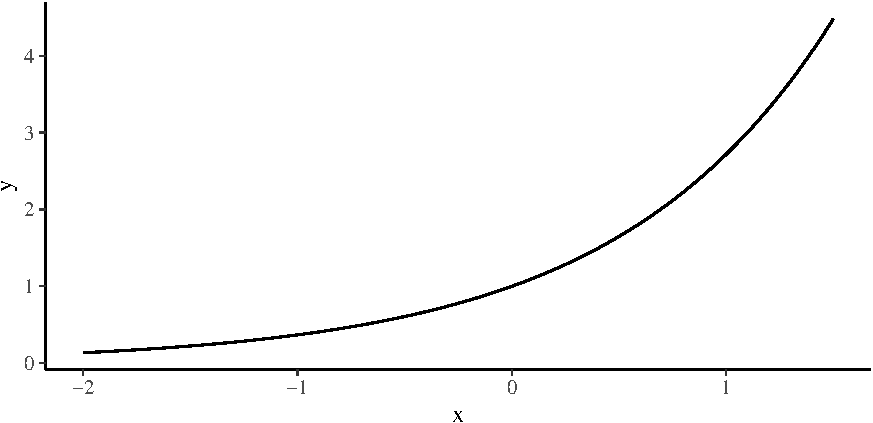
\includegraphics{045_summarize_posterior_files/figure-latex/unnamed-chunk-4-1} \end{center}

\hypertarget{stime-puntuali-della-distribuzione-a-posteriori}{%
\subsection{Stime puntuali della distribuzione a posteriori}\label{stime-puntuali-della-distribuzione-a-posteriori}}

Una volta trovata l'intera distribuzione a posteriori, quale valore di
sintesi è necessario riportare? Questa sembra una domanda innocente, ma
in realtà è una domanda a cui è difficile rispondere. La stima bayesiana dei parametri è fornita dall'intera distribuzione a posteriori, che non è un singolo numero, ma una funzione che mappa ciascun valore del parametro ad un valore di plausibilità. Quindi non è necessario scegliere una stima puntuale. In linea di principio, una stima puntuale non è quasi mai necessaria ed è spesso dannosa in quanto comporta una perdita di informazioni.

Tuttavia talvolta una tale sintesi è richiesta. Diverse risposte sono allora possibili. La media della distribuzione a posteriori per \(\theta\) è
\[
\E(\pi \mid y = 17) = \frac{\alpha}{\alpha + \beta} = \frac{25}{25+15} = 0.625.
\]
Una stima del massimo della probabilità a posteriori, o brevemente massimo a posteriori, MAP (da \emph{maximum a posteriori probability}), è la moda della distribuzione a posteriori. Nel caso presente, una stima del MAP può essere ottenuta nel modo seguente:
\[
\Mo(\pi \mid y = 17) = \frac{\alpha-1}{\alpha + \beta-2} = \frac{25-1}{25+15-2} = 0.6316.
\]
Gli stessi risultati si ottiengono usando la chiamata a \texttt{bayesrules::summarize\_beta\_binomial()}:

\begin{Shaded}
\begin{Highlighting}[]
\FunctionTok{summarize\_beta\_binomial}\NormalTok{(}\AttributeTok{alpha =} \DecValTok{8}\NormalTok{, }\AttributeTok{beta =} \DecValTok{2}\NormalTok{, }\AttributeTok{y =} \DecValTok{17}\NormalTok{, }\AttributeTok{n =} \DecValTok{30}\NormalTok{)}
\CommentTok{\#\textgreater{}       model alpha beta  mean      mode         var}
\CommentTok{\#\textgreater{} 1     prior     8    2 0.800 0.8750000 0.014545455}
\CommentTok{\#\textgreater{} 2 posterior    25   15 0.625 0.6315789 0.005716463}
\CommentTok{\#\textgreater{}          sd}
\CommentTok{\#\textgreater{} 1 0.1206045}
\CommentTok{\#\textgreater{} 2 0.0756073}
\end{Highlighting}
\end{Shaded}

La mediana si ottiene con

\begin{Shaded}
\begin{Highlighting}[]
\FunctionTok{qbeta}\NormalTok{(.}\DecValTok{5}\NormalTok{, }\AttributeTok{shape1 =} \DecValTok{25}\NormalTok{, }\AttributeTok{shape2 =} \DecValTok{15}\NormalTok{)}
\CommentTok{\#\textgreater{} [1] 0.6271031}
\end{Highlighting}
\end{Shaded}

\hypertarget{intervallo-di-credibilituxe0-1}{%
\subsection{Intervallo di credibilità}\label{intervallo-di-credibilituxe0-1}}

È più comune sintetizzare la distribuzione a posteriori mediante l'intervallo di credibilità. Per esempio, l'intervallo di credibilità a code uguali al 95\%

\begin{Shaded}
\begin{Highlighting}[]
\FunctionTok{plot\_beta\_ci}\NormalTok{(}\AttributeTok{alpha =} \DecValTok{25}\NormalTok{, }\AttributeTok{beta =} \DecValTok{15}\NormalTok{, }\AttributeTok{ci\_level =} \FloatTok{0.95}\NormalTok{)}
\end{Highlighting}
\end{Shaded}

\begin{center}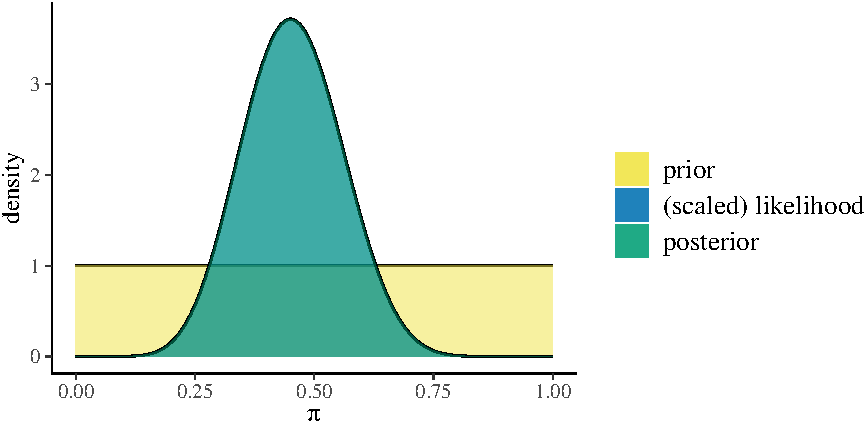
\includegraphics{045_summarize_posterior_files/figure-latex/unnamed-chunk-7-1} \end{center}

\noindent
è dato dalla chiamata

\begin{Shaded}
\begin{Highlighting}[]
\FunctionTok{qbeta}\NormalTok{(}\FunctionTok{c}\NormalTok{(}\FloatTok{0.025}\NormalTok{, }\FloatTok{0.975}\NormalTok{), }\DecValTok{25}\NormalTok{, }\DecValTok{15}\NormalTok{)}
\CommentTok{\#\textgreater{} [1] 0.4717951 0.7663607}
\end{Highlighting}
\end{Shaded}

\noindent
Il calcolo precedente evidenzia l'interpretazione intuitiva dell'intervallo di credibilità. Tale intervallo, infatti, può essere interpretato come la probabilità che \(\theta\) assuma valori compresi tra 0.472 e 0.766:
\[
P(\theta \in (0.472, 0.766) | Y = 17) = \int_{0.472}^{0.766} f(\theta \mid y=17) d\theta = 0.95,
\]
ovvero

\begin{Shaded}
\begin{Highlighting}[]
\NormalTok{postFun }\OtherTok{\textless{}{-}} \ControlFlowTok{function}\NormalTok{(theta) \{}
  \FunctionTok{gamma}\NormalTok{(}\DecValTok{25} \SpecialCharTok{+} \DecValTok{15}\NormalTok{) }\SpecialCharTok{/}\NormalTok{ (}\FunctionTok{gamma}\NormalTok{(}\DecValTok{25}\NormalTok{) }\SpecialCharTok{*} \FunctionTok{gamma}\NormalTok{(}\DecValTok{15}\NormalTok{)) }\SpecialCharTok{*}\NormalTok{ theta}\SpecialCharTok{\^{}}\DecValTok{24} \SpecialCharTok{*}\NormalTok{ (}\DecValTok{1} \SpecialCharTok{{-}}\NormalTok{ theta)}\SpecialCharTok{\^{}}\DecValTok{14}
\NormalTok{\}}
\FunctionTok{integrate}\NormalTok{(}
\NormalTok{  postFun,}
  \AttributeTok{lower =} \FloatTok{0.4717951}\NormalTok{,}
  \AttributeTok{upper =} \FloatTok{0.7663607}
\NormalTok{)}\SpecialCharTok{$}\NormalTok{value}
\CommentTok{\#\textgreater{} [1] 0.95}
\end{Highlighting}
\end{Shaded}

Possiamo costruire diversi intervalli di credibilità a code equivalenti. Ad esempio, l'intervallo di credibilità compreso tra il 25-esimo e il 75-esimo percentile è

\begin{Shaded}
\begin{Highlighting}[]
\FunctionTok{qbeta}\NormalTok{(}\FunctionTok{c}\NormalTok{(}\FloatTok{0.25}\NormalTok{, }\FloatTok{0.75}\NormalTok{), }\DecValTok{25}\NormalTok{, }\DecValTok{15}\NormalTok{)}
\CommentTok{\#\textgreater{} [1] 0.5743878 0.6778673}
\end{Highlighting}
\end{Shaded}

\noindent
ovvero, abbiamo una certezza a posteriori del 50\% che la probabilità di depressione grave tra i pazienti clinici sia un valore compreso tra 0.57 e 0.68.

Non esiste un livello credibile ``corretto''. I ricercatori, utilizzano vari livelli, ad esempio 50\%, 80\% o 95\%, a seconda del contesto dell'analisi. Ciascuno di questi intervalli fornisce un'immagine diversa della nostra comprensione della distribuzione a posteriori del parametro di interesse.

Non è inoltre necessario riportare l'intervallo di credibilità a code uguali. Se la distribuzione a posteriori è fortemente asimmetrica è più sensato riportare l'intervallo di credibilità a densità a posteriori più alta.
L'intervallo HPD risulta più semplice da determinare quando la distribuzione a posteriori viene approssimata con il metodo MCMC.

\hypertarget{probabilituxe0-della-distribuzione-a-posteriori}{%
\subsection{Probabilità della distribuzione a posteriori}\label{probabilituxe0-della-distribuzione-a-posteriori}}

Il test di ipotesi è un compito comune dell'analisi della distribuzione a posteriori. Supponiamo che si voglia conoscere la probabilità a posteriori che \(\theta\) sia superiore a 0.5. Per sapere quanto credibile sia l'evento \(\theta > 0.5\) possiamo calcolare il seguente integrale:
\[
P(\theta > 0.5 \; \mid \; y = 17) = \int_{0.5}^{1}f(\theta \mid y=17)d\theta \;,
\]
dove \(f(\cdot)\) è la distribuzione \(\mbox{\Beta}(25, 15)\):

\begin{Shaded}
\begin{Highlighting}[]
\FunctionTok{pbeta}\NormalTok{(}\FloatTok{0.5}\NormalTok{, }\AttributeTok{shape1 =} \DecValTok{25}\NormalTok{, }\AttributeTok{shape2 =} \DecValTok{15}\NormalTok{, }\AttributeTok{lower.tail =} \ConstantTok{FALSE}\NormalTok{)}
\CommentTok{\#\textgreater{} [1] 0.9459355}
\end{Highlighting}
\end{Shaded}

\noindent
il che è equivalente a:

\begin{Shaded}
\begin{Highlighting}[]
\NormalTok{postFun }\OtherTok{\textless{}{-}} \ControlFlowTok{function}\NormalTok{(theta) \{}
  \FunctionTok{gamma}\NormalTok{(}\DecValTok{25} \SpecialCharTok{+} \DecValTok{15}\NormalTok{) }\SpecialCharTok{/}\NormalTok{ (}\FunctionTok{gamma}\NormalTok{(}\DecValTok{25}\NormalTok{) }\SpecialCharTok{*} \FunctionTok{gamma}\NormalTok{(}\DecValTok{15}\NormalTok{)) }\SpecialCharTok{*}\NormalTok{ theta}\SpecialCharTok{\^{}}\DecValTok{24} \SpecialCharTok{*}\NormalTok{ (}\DecValTok{1} \SpecialCharTok{{-}}\NormalTok{ theta)}\SpecialCharTok{\^{}}\DecValTok{14}
\NormalTok{\}}
\FunctionTok{integrate}\NormalTok{(}
\NormalTok{  postFun,}
  \AttributeTok{lower =} \FloatTok{0.5}\NormalTok{,}
  \AttributeTok{upper =} \DecValTok{1}
\NormalTok{)}\SpecialCharTok{$}\NormalTok{value}
\CommentTok{\#\textgreater{} [1] 0.9459355}
\end{Highlighting}
\end{Shaded}

È anche possibile formulare un test di ipotesi contrastando due ipotesi contrapposte. Per esempio, \(H_1: \theta \geq 0.5\) e \(H_2: \theta < 0.5\). Ciò consente di calcolare l'\emph{odds a posteriori} di \(\theta > 0.5\):
\begin{equation}
\text{poterior odds} = \frac{H_1 \mid y = 17}{H_2 \mid y = 17}
\end{equation}
ovvero

\begin{Shaded}
\begin{Highlighting}[]
\NormalTok{posterior\_odds }\OtherTok{\textless{}{-}}
  \FunctionTok{pbeta}\NormalTok{(}\FloatTok{0.5}\NormalTok{, }\AttributeTok{shape1 =} \DecValTok{25}\NormalTok{, }\AttributeTok{shape2 =} \DecValTok{15}\NormalTok{, }\AttributeTok{lower.tail =} \ConstantTok{FALSE}\NormalTok{) }\SpecialCharTok{/}
    \FunctionTok{pbeta}\NormalTok{(}\FloatTok{0.5}\NormalTok{, }\AttributeTok{shape1 =} \DecValTok{25}\NormalTok{, }\AttributeTok{shape2 =} \DecValTok{15}\NormalTok{, }\AttributeTok{lower.tail =} \ConstantTok{TRUE}\NormalTok{)}
\NormalTok{posterior\_odds}
\CommentTok{\#\textgreater{} [1] 17.49642}
\end{Highlighting}
\end{Shaded}

\noindent
L'odds a posteriori rappresenta l'aggiornamento delle nostre credenze dopo avere osservato \(y = 17\) in \(n = 30\). L'odds a priori di \(\theta > 0.5\) era:

\begin{Shaded}
\begin{Highlighting}[]
\NormalTok{prior\_odds }\OtherTok{\textless{}{-}}
  \FunctionTok{pbeta}\NormalTok{(}\FloatTok{0.5}\NormalTok{, }\AttributeTok{shape1 =} \DecValTok{8}\NormalTok{, }\AttributeTok{shape2 =} \DecValTok{2}\NormalTok{, }\AttributeTok{lower.tail =} \ConstantTok{FALSE}\NormalTok{) }\SpecialCharTok{/}
    \FunctionTok{pbeta}\NormalTok{(}\FloatTok{0.5}\NormalTok{, }\AttributeTok{shape1 =} \DecValTok{8}\NormalTok{, }\AttributeTok{shape2 =} \DecValTok{2}\NormalTok{, }\AttributeTok{lower.tail =} \ConstantTok{TRUE}\NormalTok{)}
\NormalTok{prior\_odds}
\CommentTok{\#\textgreater{} [1] 50.2}
\end{Highlighting}
\end{Shaded}

Il \emph{fattore di Bayes} (\emph{Bayes Factor}; BF) confronta gli odds a posteriori con gli odds a priori e quindi fornisce informazioni su quanto sia mutata la nostra comprensione relativa a \(\theta\) dopo avere osservato i nostri dati del campione:
\[
\text{BF} = \frac{\text{odds a posteriori}}{\text{odds a priori}}.
\]
Nel caso presente abbiamo

\begin{Shaded}
\begin{Highlighting}[]
\NormalTok{BF }\OtherTok{\textless{}{-}}\NormalTok{ posterior\_odds }\SpecialCharTok{/}\NormalTok{ prior\_odds}
\NormalTok{BF}
\CommentTok{\#\textgreater{} [1] 0.3485343}
\end{Highlighting}
\end{Shaded}

Quindi, dopo avere osservato i dati, gli odds a posteriori della nostra ipotesi a proposito di \(\theta\) sono pari a solo il 34\% degli odds a priori.

Per fare un altro esempio, consideriamo invece il caso in cui le credenze a priori rivelano una credenza diametralmente opposta rispetto a \(\theta\) che nel caso considerato in precedenza, ovvero \(\mbox{Beta}(2, 8)\). In questo secondo caso, la distribuzione a posteriori diventa

\begin{Shaded}
\begin{Highlighting}[]
\FunctionTok{summarize\_beta\_binomial}\NormalTok{(}\AttributeTok{alpha =} \DecValTok{2}\NormalTok{, }\AttributeTok{beta =} \DecValTok{8}\NormalTok{, }\AttributeTok{y =} \DecValTok{17}\NormalTok{, }\AttributeTok{n =} \DecValTok{30}\NormalTok{)}
\CommentTok{\#\textgreater{}       model alpha beta  mean      mode         var}
\CommentTok{\#\textgreater{} 1     prior     2    8 0.200 0.1250000 0.014545455}
\CommentTok{\#\textgreater{} 2 posterior    19   21 0.475 0.4736842 0.006082317}
\CommentTok{\#\textgreater{}           sd}
\CommentTok{\#\textgreater{} 1 0.12060454}
\CommentTok{\#\textgreater{} 2 0.07798921}
\end{Highlighting}
\end{Shaded}

\noindent
e il BF è

\begin{Shaded}
\begin{Highlighting}[]
\NormalTok{posterior\_odds }\OtherTok{\textless{}{-}}
  \FunctionTok{pbeta}\NormalTok{(}\FloatTok{0.5}\NormalTok{, }\AttributeTok{shape1 =} \DecValTok{19}\NormalTok{, }\AttributeTok{shape2 =} \DecValTok{21}\NormalTok{, }\AttributeTok{lower.tail =} \ConstantTok{FALSE}\NormalTok{) }\SpecialCharTok{/}
    \FunctionTok{pbeta}\NormalTok{(}\FloatTok{0.5}\NormalTok{, }\AttributeTok{shape1 =} \DecValTok{19}\NormalTok{, }\AttributeTok{shape2 =} \DecValTok{21}\NormalTok{, }\AttributeTok{lower.tail =} \ConstantTok{TRUE}\NormalTok{)}

\NormalTok{prior\_odds }\OtherTok{\textless{}{-}}
  \FunctionTok{pbeta}\NormalTok{(}\FloatTok{0.5}\NormalTok{, }\AttributeTok{shape1 =} \DecValTok{2}\NormalTok{, }\AttributeTok{shape2 =} \DecValTok{8}\NormalTok{, }\AttributeTok{lower.tail =} \ConstantTok{FALSE}\NormalTok{) }\SpecialCharTok{/}
    \FunctionTok{pbeta}\NormalTok{(}\FloatTok{0.5}\NormalTok{, }\AttributeTok{shape1 =} \DecValTok{2}\NormalTok{, }\AttributeTok{shape2 =} \DecValTok{8}\NormalTok{, }\AttributeTok{lower.tail =} \ConstantTok{TRUE}\NormalTok{)}

\NormalTok{BF }\OtherTok{\textless{}{-}}\NormalTok{ posterior\_odds }\SpecialCharTok{/}\NormalTok{ prior\_odds}
\NormalTok{BF}
\CommentTok{\#\textgreater{} [1] 30.07239}
\end{Highlighting}
\end{Shaded}

\noindent
In alre parole, in questo secondo esempio gli odds a posteriori della nostra ipotesi a proposito di \(\theta\) sono aumentati di 30 volte rispetto agli odds a priori.

In generale, in un test di ipotesi che contrappone un'ipotesi sostantiva \(H_a\) ad un'ipotesi nulla \(H_0\) il BF è un rapporto di odds per l'ipotesi sostantiva:
\[
\text{Bayes Factor}
= \frac{\text{posterior odds}}{\text{prior odds}}
= \frac{P(H_a \mid Y) / P(H_0 \mid Y)}{P(H_a) / P(H_0)}
 \; .
\]
Essendo un rapporto, il BF deve esere valutato rispetto al valore di 1. Ci sono tre possibilità:

\begin{itemize}
\tightlist
\item
  BF = 1: La credibilità di \(H_a\) non è cambiata dopo avere osservato i dati.
\item
  BF \textgreater{} 1: La credibilità di \(H_a\) è aumentata dopo avere osservato i dati. Quindi maggiore è BF, più convincente risulta l'evidenza per \(H_a\).
\item
  BF \textless{} 1: La credibilità di \(H_a\) è diminuita dopo avere osservato i dati.
\end{itemize}

Non ci sono delle soglie universalmente riconosciute per interpretare il BF. Per esempio, \textcite{lee2014bayesian} propongono il seguente schema:

\begin{longtable}[]{@{}rl@{}}
\toprule
BF & Interpretation \\
\midrule
\endhead
\textgreater{} 100 & Extreme evidence for \(H_a\) \\
30 - 100 & Very strong evidence for \(H_a\) \\
10 - 30 & Strong evidence for \(H_a\) \\
3 - 10 & Moderate evidence for \(H_a\) \\
1 - 3 & Anecdotal evidence for \(H_a\) \\
1 & No evidence \\
1/3 - 1 & Anecdotal evidence for \(H_0\) \\
1/10 - 1/3 & Moderate evidence for \(H_0\) \\
1/30 - 1/10 & Strong evidence for \(H_0\) \\
1/100 - 1/30 & Very strong evidence for \(H_0\) \\
\textless{} 1/100 & Extreme evidence for \(H_0\) \\
\bottomrule
\end{longtable}

Tuttavia, è importante notare che l'opinione maggiormente diffusa nella comunità scientifica sia quella che incoraggia a non trarre conclusioni rigide dai dati utilizzando dei criteri fissati una volta per tutte. Pertanto, non esiste una soglia univoca per il BF che consente di classificare le ipotesi dei ricercatori nelle due categorie ``vero'' o ``falso''. Invece, è più utile adottare una pratica più flessibile capace di tenere in considerazione il contesto e le potenziali implicazioni di ogni singolo test di ipotesi. Inoltre, è stato molte volte ripetuto che la distribuzione a posteriori è molto più informativa di una decisione binaria: la rappresentazione di tutta la distribuzione a posteriori fornisce una misura olistica del nostro livello di incertezza riguardo all'affermazione (il parametro, ovvero l'ipotesi) che viene valutata.

\hypertarget{considerazioni-conclusive}{%
\section*{Considerazioni conclusive}\label{considerazioni-conclusive}}
\addcontentsline{toc}{section}{Considerazioni conclusive}

Questo capitolo introduce le procedure di base per la manipolazione
della distribuzione a posteriori. Lo strumento fondamentale che è stato
utilizzato è quello fornito dai campioni di valori del parametro che vengono estratti dalla distribuzione a posteriori. Lavorare con campioni di valori del parametro estratti dalla distribuzione a posteriori trasforma un problema di calcolo integrale in un problema di riepilogo dei dati. Abbiamo visto le procedure maggiormente usate che consentono di utilizzare i campioni a
posteriori per produrre indici di sintesi della distribuzione a
posteriori: gli intervalli di credibilità e le stime puntuali.


% Bibliography
%%%%%%%%%%%%%%%%%%%%%%%%%%%%%%%%%%%%%%%%%%%%%%%%%%%%%%%%%%

\backmatter
\SmallMargins

\printbibliography
\onecolumn


% Tables (of tables, of figures)
%%%%%%%%%%%%%%%%%%%%%%%%%%%%%%%%%%%%%%%%%%%%%%%%%%%%%%%%%%


\cleardoublepage
\LargeMargins
\listoffigures


% After-body (LaTeX code inclusion)
%%%%%%%%%%%%%%%%%%%%%%%%%%%%%%%%%%%%%%%%%%%%%%%%%%%%%%%%%%




% Back cover
%%%%%%%%%%%%%%%%%%%%%%%%%%%%%%%%%%%%%%%%%%%%%%%%%%%%%%%%%%%

% Even page, small margins, no running head, no page number.
\evenpage
\SmallMargins
\thispagestyle{empty}

\begin{normalsize}

\begin{description}

\selectlanguage{italian}
\item[Abstract]
This document contains the material of the lessons of Psicometria B000286 (2021/2022) aimed at students of the first year of the Degree Course in Psychological Sciences and Techniques of the University of Florence, Italy.
\item[Keywords]
Data science, Bayesian statistics.
~\\

\end{description}

\end{normalsize}


\end{document}
